\documentclass[12pt]{article}


\usepackage[utf8]{inputenc}
\usepackage[a4paper,top=3cm,bottom=2cm,left=3cm,right=3cm,marginparwidth=1.75cm]{geometry}
\usepackage[nodayofweek]{datetime}
\usepackage{tabularx}
\usepackage[small]{titlesec}
\usepackage{graphicx}
\usepackage{tabularx}
\usepackage{fancyvrb}
\usepackage{upgreek}
\newcolumntype{L}[1]{>{\raggedright\arraybackslash}p{#1}}
\newcolumntype{C}[1]{>{\centering\arraybackslash}p{#1}}
\newcolumntype{R}[1]{>{\raggedleft\arraybackslash}p{#1}}

\begin{document}

\begin{titlepage}
    \begin{center}
        \huge{\bfseries  Tribhuvan University}\\
        \Large{Institute of Engineering}\\
        \huge{ \bfseries  Pulchowk Campus}\\[3.2cm]


        \textsc{\Large Digital Signal Analysis and Processing}\\[-0.5cm]
        \line(1,0){400}\\
        \huge{\bfseries Lab 2}\\
        \huge{Basic CT/DT functions}
        \line(1,0){400}\\


        \textsc{\Large Submitted by:}\\
        \Large Bishal Katuwal\\ \large 075BCT028\\    [0.85cm]

        \textsc{\Large Submitted to:}\\\
        \large Department of Electronics and Computer Engineering\\Pulchowk Campus\\    [0.85cm]
        
        \textsc{\Large Submitted on:}\\
        \today
        
    \end{center}
\end{titlepage}
\pagebreak
% ===============================================================
\paragraph{Title\\}
Basic CT/DT functions
\paragraph{Background Theory}
\subparagraph{Continuous Time Signal\\}
A continuous time signal is a function that is continuous, meaning there are no breaks in the signal. 
For all real values of t, f(t) exists.
CT signals are ususally represented by using x(t), having a parentheses and the variable t.
\begin{figure}[h!]
    \centering
    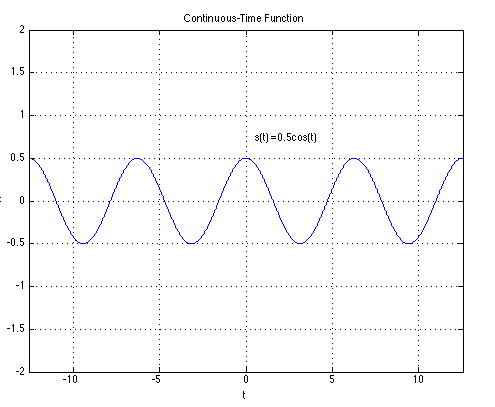
\includegraphics[scale = 0.5]{labss/Lab2_Th_CT.PNG}
    \caption{CT Signals}
\end{figure}
\subparagraph{Discrete Time Signals\\}
A discrete time signal is a signal whose value is taken at discrete measurements.
For discrete time signal, the function exists only at a certain interval of timr. 
Thus there will be time periods of n where F(n) doesn't have a value. 
DT signals are represented using the form x[n]. 
Discrete signals are the approximations of CT signals
\begin{figure}[h!]
    \centering
    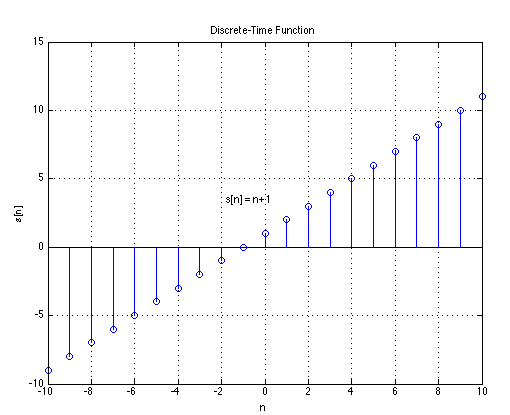
\includegraphics[scale = 0.6]{labss/Lab2_Th_DT.PNG}
    \caption{DT Signals}
\end{figure}
\subparagraph{Some basic CT/DT functions}
\begin{itemize}
    \item Sinusoidal function\\
    Trig functions like sine and cosine have periodic graphs which we called Sinusoidal Graph, or Sine wave.
    \begin{figure}[h!]
        \centering
        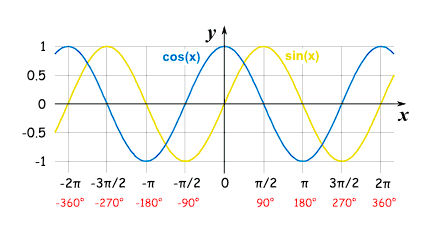
\includegraphics{labss/Lab2_TH_Sine.PNG}
        \caption{Sine and cosine wave}
    \end{figure}
    They’re three features of sinusoidal graphs.
    \begin{itemize}
        \item  {\bfseries Midline}: is the horizontal line that passes exactly in the middle between the graph's maximum and minimum points.
        \item {\bfseries Amplitude}: is the vertical distance between the midline and one of the extremum points.
        \item {\bfseries Period}: Also called frequency, is the distance between two consecutive maximum points, or two consecutive minimum points (these distances must be equal).
    \end{itemize}
    \begin{figure}[h!]
        \centering
        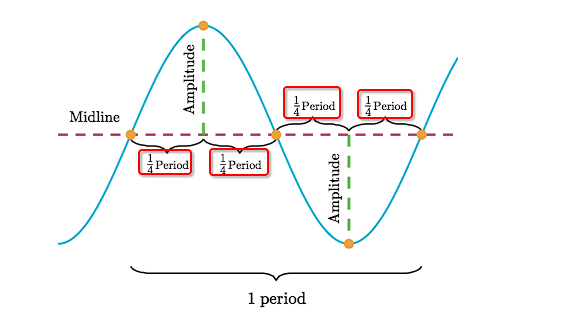
\includegraphics[scale = 0.7]{labss/Lab2_TH_Sine_Props.PNG}
        \caption{Sinusoidal wave features} 
    \end{figure}
    In MATLAB. sinusoidal functions can simply be called as 
    \begin{verbatim}
        sin(x)
        cos(x)
    \end{verbatim}
    
    \item Ramp function\\
    The ramp function is a unary real function, whose graph is shaped like a ramp. 
    In this lab, ramp function denotes the unit ramp function (slope 1, starting at 0).
    \begin{figure}[h!]
        \centering
        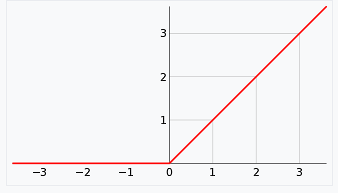
\includegraphics[scale = 0.7]{labss/Lab2_TH_Ramp.PNG}
        \caption{Ramp wave} 
    \end{figure}\\
    In MATLAB. ramp functions can simply be called as 
    \begin{verbatim}
        ramp(x)
    \end{verbatim}
    \item Exponential function\\
    An exponential function is simply a function in which the independent variable is the exponent.
    Exponential function is defined as:
    \begin{Verbatim}
    If b is any number such that b > 0 and b != 1 then,
    an exponential function is a function in the form,
    f(x) =b^x
    where 
    b is called the base and 
    x can be any real number.
    \end{Verbatim}
    Exponential functions can be increasing or decreasing.
    \begin{figure}[h!]
        \centering
        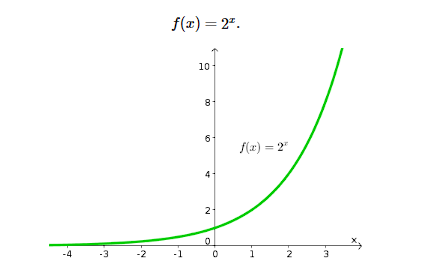
\includegraphics[scale = 0.7]{labss/Lab2_TH_Exp_inc.PNG}
        \caption{Increasing exponential function} 
    \end{figure}\\

    \begin{figure}[h!]
        \centering
        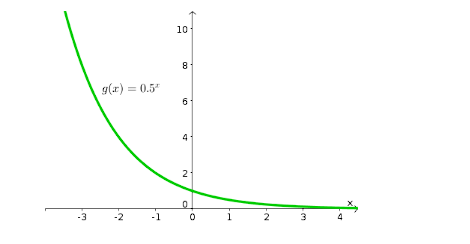
\includegraphics[scale = 0.7]{labss/Lab2_TH_Exp_dec.PNG}
        \caption{Decreasing exponential function} 
    \end{figure}
    \pagebreak
    In MATLAB. exponential functions can simply be called as 
    \begin{verbatim}
        exp(x)
    \end{verbatim}
    \item Unit step function\\
    The unit step function is a function whose is zero for negative arguments and one for positive arguments.
    \begin{figure}[h!]
        \centering
        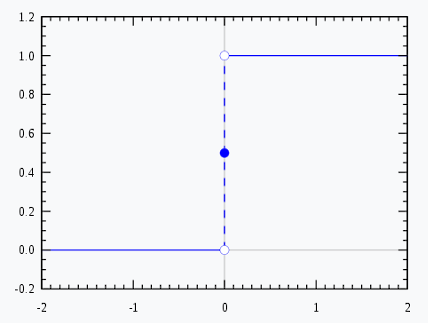
\includegraphics[scale = 0.7]{labss/Lab2_TH_Step.PNG}
        \caption{Unit Step function} 
    \end{figure}\\
    In MATLAB. unit step functions can simply be called as 
    \begin{verbatim}
        heaviside(x)
    \end{verbatim}
    \pagebreak
    \item Unit impulse functions\\
    The unit impulse function is a function whose is one for 0 as argument and zero for all other arguments.
    \begin{figure}[h!]
        \centering
        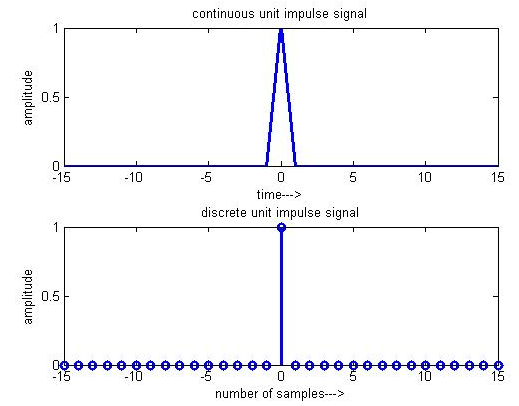
\includegraphics[scale = 0.7]{labss/Lab2_TH_Impulse.PNG}
        \caption{Unit Impulse function} 
    \end{figure}\\
    In MATLAB. unit impulse functions can simply be called as 
    \begin{verbatim}
        dirac(x)
    \end{verbatim}
\end{itemize}
% =============================================
\pagebreak
\paragraph{Activity}
\begin{enumerate}
    \item Sinusoidal signals
    \begin{itemize}
        \item Continuous Sine wave \:
        \begin{Verbatim}[frame = single]
t = -10:0.01:10
x = sin(t)
plot(t,x)
xlabel('t')
ylabel('x')
title(sinosoidal)
        \end{Verbatim}
        \begin{figure}[h!]
            \centering
            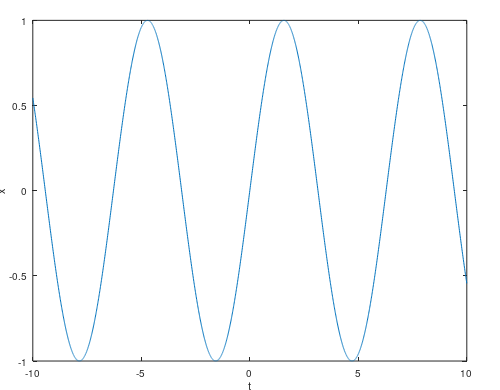
\includegraphics[scale =0.4]{labss/Lab2_1a.PNG}
            \caption{Continuous sine wave}
        \end{figure}
        \item Discrete Sine wave \:
        \begin{Verbatim}[frame = single]
t = -10:0.5:10
x = sin(t)
stem(t,x)
xlabel('t')
ylabel('x')
title(sinosoidal)
        \end{Verbatim}
        \begin{figure}[h!]
            \centering
            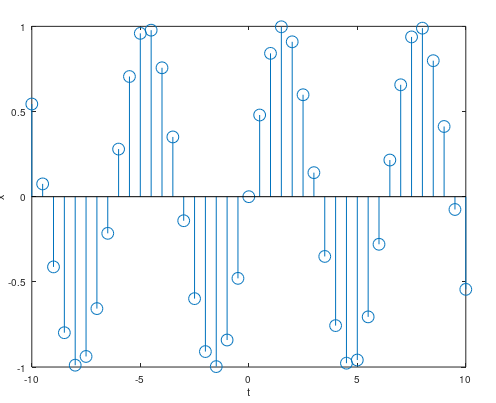
\includegraphics[scale =0.55]{labss/Lab2_1b.PNG}
            \caption{Discrete sine wave}
        \end{figure}
        \item Sine wave with hold on \:
        \begin{Verbatim}[frame = single]
t = -10:0.01:10
x = sin(t)
y=cos(t)
plot(t,x)
hold on
plot(t,y)
hold off
        \end{Verbatim}
        \begin{figure}[h!]
            \centering
            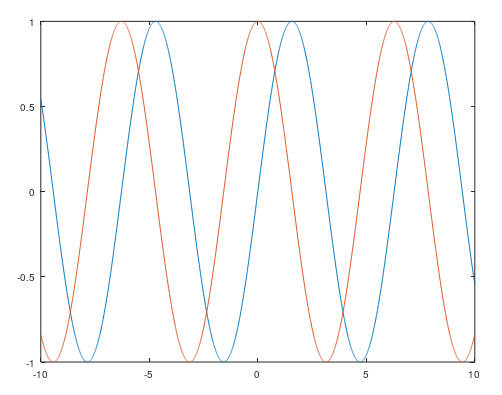
\includegraphics[scale =0.7]{labss/Lab2_1c.PNG}
            \caption{sine wave and cosine wave}
        \end{figure}
        \pagebreak
    \end{itemize}

    \item Ramp signals
    \begin{Verbatim}[frame = single]
x= -10:10
y=x
plot(x,y)
                \end{Verbatim}
                \begin{figure}[h!]
                    \centering
                    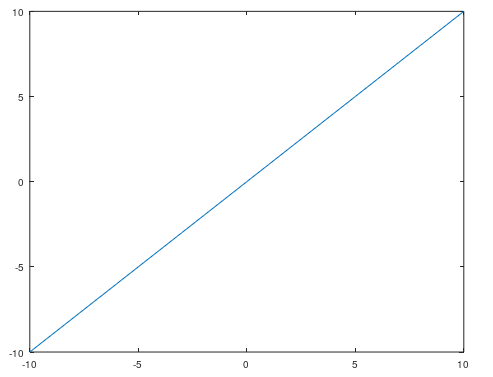
\includegraphics[scale =0.7]{labss/Lab2_2a.PNG}
                    \caption{Ramp wave}
                \end{figure}
                \pagebreak

    \item Exponential signals
    \begin{itemize}
        
        \item Exponentially growing \:
        \begin{Verbatim}[frame = single]
n= -10:10
a = 0.25
c=2
y = c*exp(a*n)
stem(n,y)
title('Éxponentiallly growing']
        \end{Verbatim}
        \begin{figure}[h!]
            \centering
            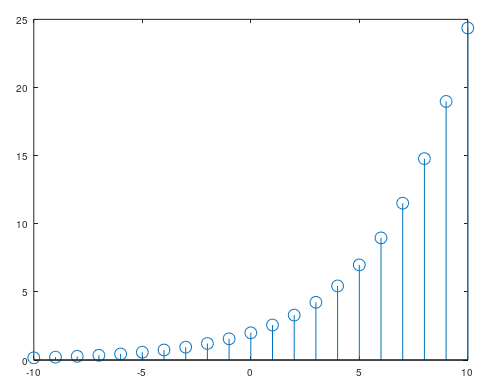
\includegraphics[scale =0.5]{labss/Lab2_3a.PNG}
            \caption{Éxponentiallly growing wave}
        \end{figure}
        
        \item Exponentially decaying wave \:
        \begin{Verbatim}[frame = single]
n= -10:10
a = -0.25
c=2
y = c*exp(a*n)
stem(n,y)
        \end{Verbatim}
        \begin{figure}[h!]
            \centering
            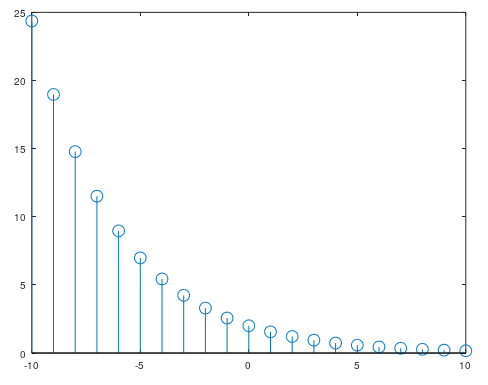
\includegraphics[scale =0.55]{labss/Lab2_3b.PNG}
            \caption{Exponentially decaying wave}
        \end{figure}
        
        \item Constant Wave\:
        \begin{Verbatim}[frame = single]
n= -10:10
a = 0
c=2
y = c*exp(a*n)
stem(n,y)
        \end{Verbatim}
        \begin{figure}[h!]
            \centering
            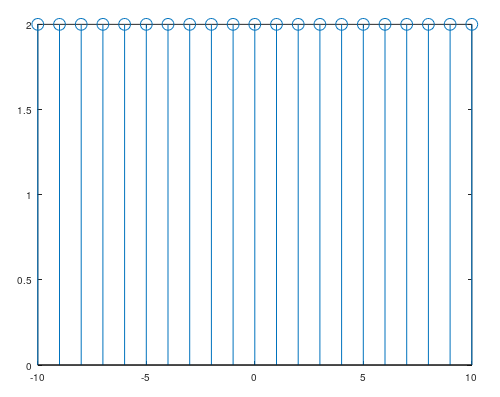
\includegraphics[scale =0.7]{labss/Lab2_3c.PNG}
            \caption{Constant wave}
        \end{figure}
        \pagebreak
    \end{itemize}

    \item Unit step signals
    \begin{Verbatim}[frame = single]
hold on
for(n =-10:10)
    if(n<0)
        stem(n,0)
    else
        stem(n,1)
    end
end
hold off
                \end{Verbatim}
                \begin{figure}[h!]
                    \centering
                    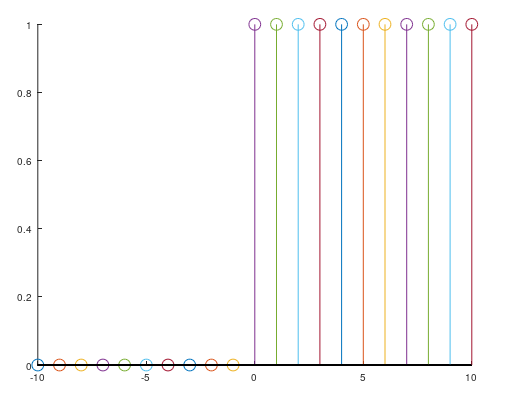
\includegraphics[scale =0.7]{labss/Lab2_4a.PNG}
                    \caption{Unit step function}
                \end{figure}
                \pagebreak
    \item Unit impulse signals
    \begin{Verbatim}[frame = single]
hold on
for(n =-10:10)
    if(n==0)
        stem(n,1)
    else
        stem(n,0)
    end
end
hold off
                        \end{Verbatim}
                        \begin{figure}[h!]
                            \centering
                            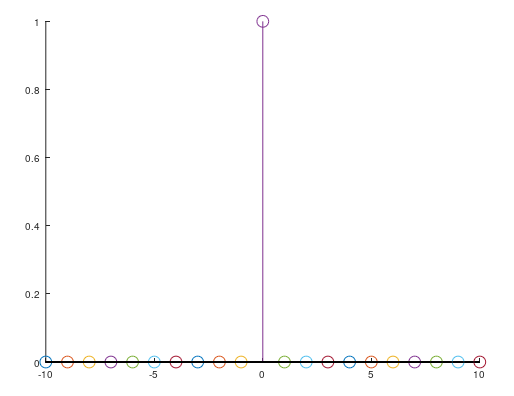
\includegraphics[scale =0.7]{labss/Lab2_5a.PNG}
                            \caption{Unit impulse function}
                        \end{figure}
\end{enumerate}
\paragraph{Conclusion\\}
In this way "Lab 2: Basic CT/DT functions" was completed via the use of MATLAB.
Five basic functions were studied.The functions were:
\begin{itemize}
    \item Sinusoidal function
    \item Ramp function
    \item Exponential function
    \item Unit step function
    \item Unit impulse function
\end{itemize}
\end{document}